% accuracy and attention comparison figures

\begin{figure*}[t!]

  \centering
  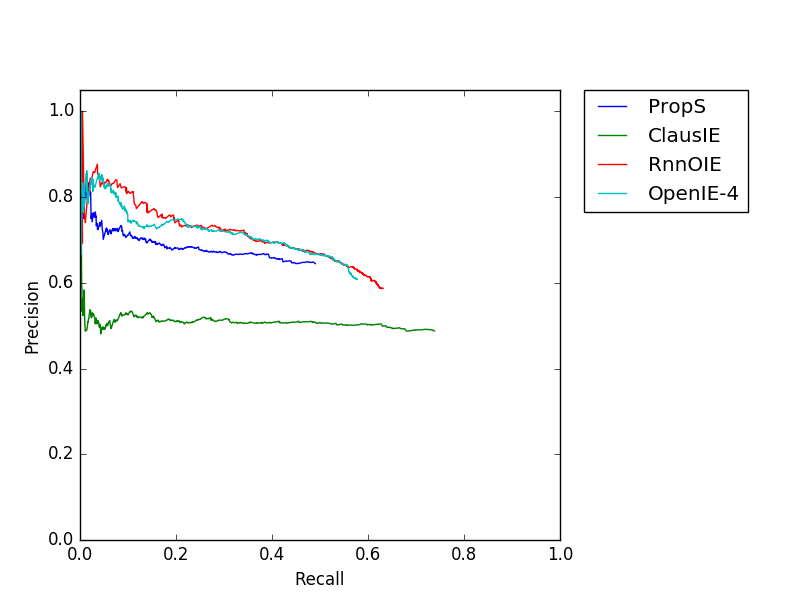
\includegraphics[width=.5\textwidth]{figures/joint/pr}\hfill
  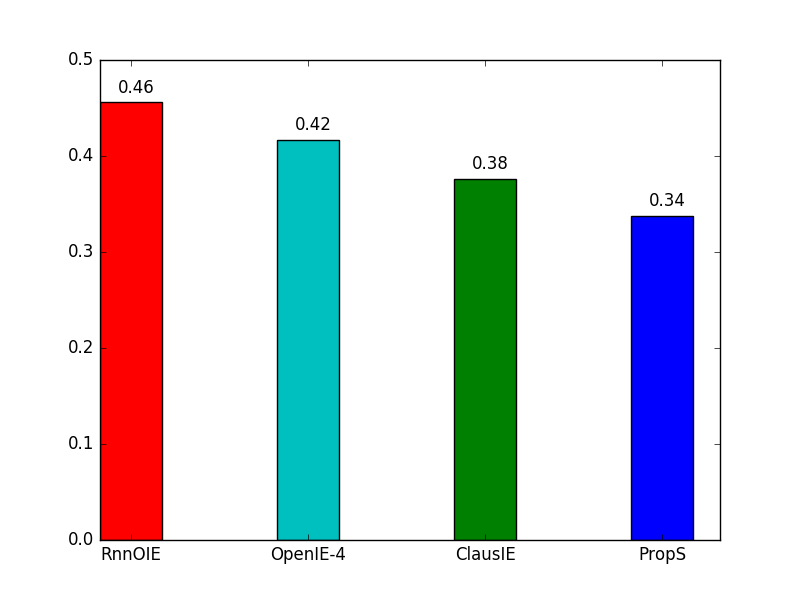
\includegraphics[width=.5\textwidth]{figures/joint/auc}

  \caption{Precision-Recall curve (left) and respective area under the curve (right) for the different systems.}
  \label{fig:evaluation}

\end{figure*}


%% \begin{figure*}[t!]

%%   \centering
%%   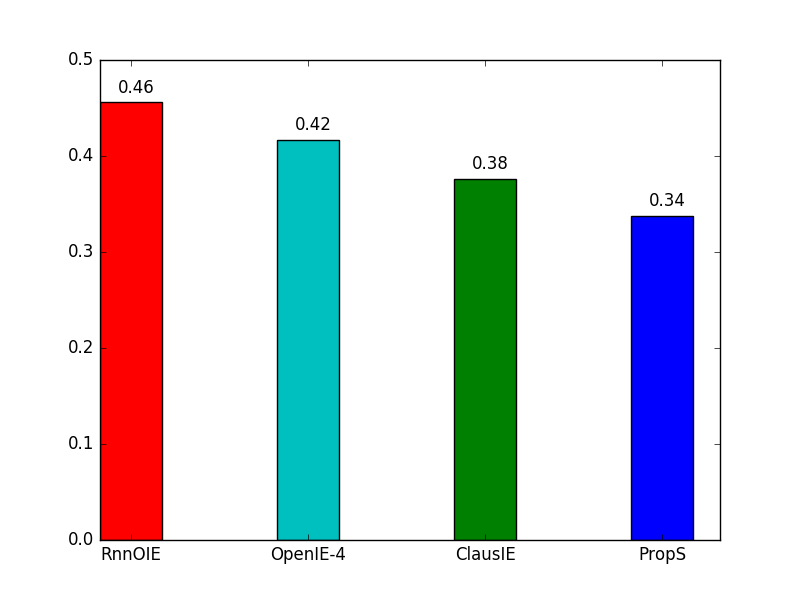
\includegraphics[width=.3\textwidth]{figures/joint/auc}\hfill
%%   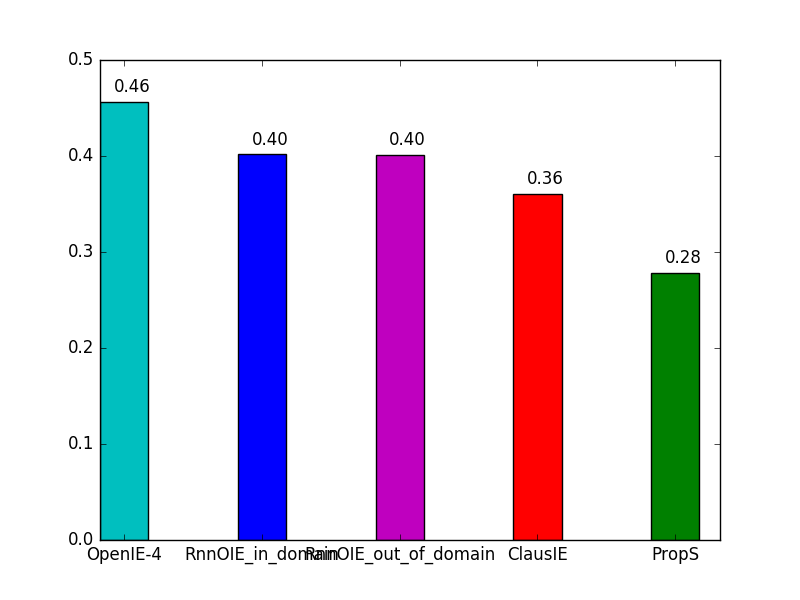
\includegraphics[width=.3\textwidth]{figures/newswire/auc}\hfill
%%     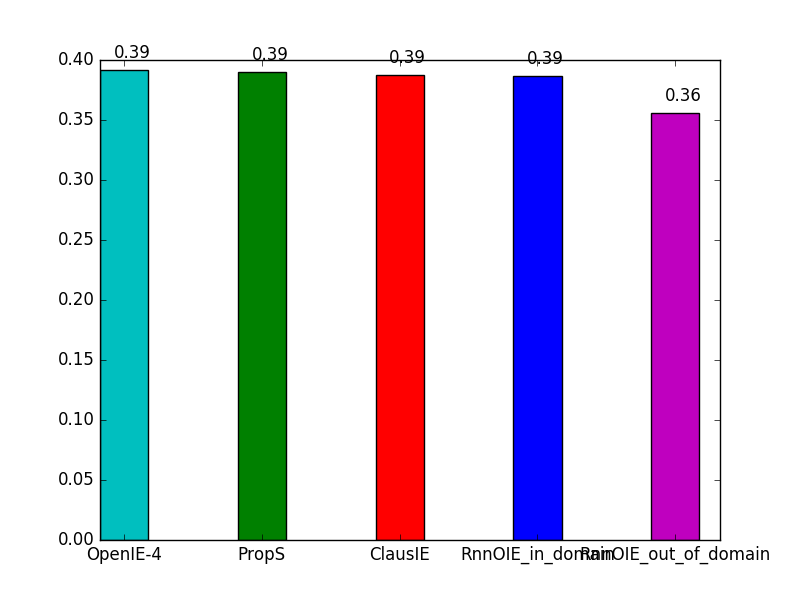
\includegraphics[width=.3\textwidth]{figures/wiki/auc}

%%   \caption{Area under the PR - curves for the entire test corpus (left), Newswire (middle), and Wikipedia (right).}
%%   \label{fig:figure3}

%% \end{figure*}



%% \begin{figure*}[!hb]

%%   \centering

%%   \begin{minipage}[b]{.12\textwidth}
%%     \begin{center}
%%       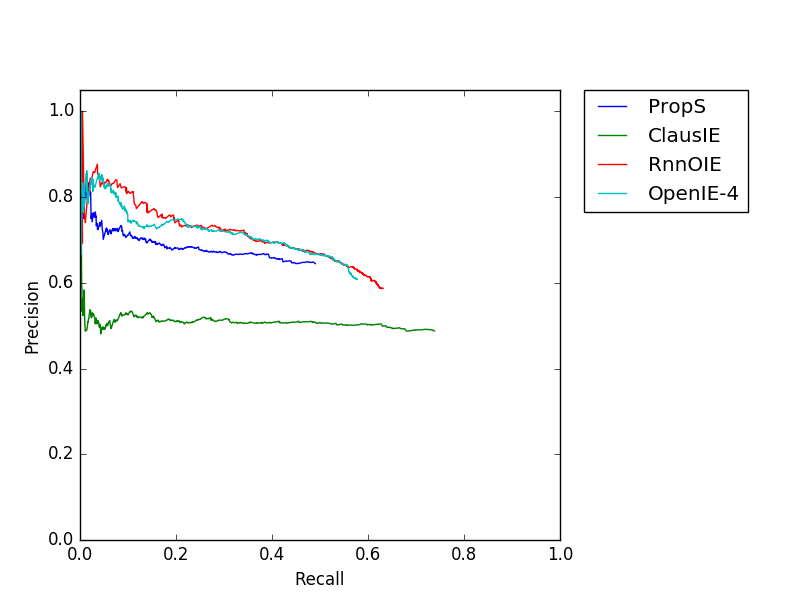
\includegraphics[width=\textwidth]{figures/joint/pr}
%%       \caption {Precision-recall curve on the full test partition}
%%       \label{fig:alignments}
%%     \end{center}
%%   \end{minipage}

%%   \begin{minipage}[b]{0.12\textwidth}
%%     \begin{center}
%%       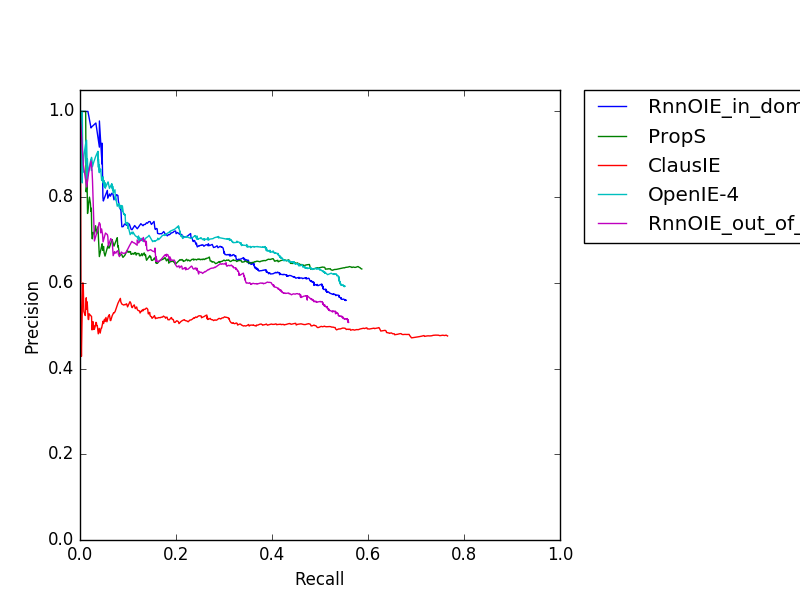
\includegraphics[width=\textwidth]{figures/wiki/pr}
%%       \caption {Precision-recall curve on the Wikipedia test partition}
%%       \label{fig:alignments}
%%     \end{center}
%%   \end{minipage}

%%   \begin{minipage}[b]{0.12\textwidth}
%%     \begin{center}
%%       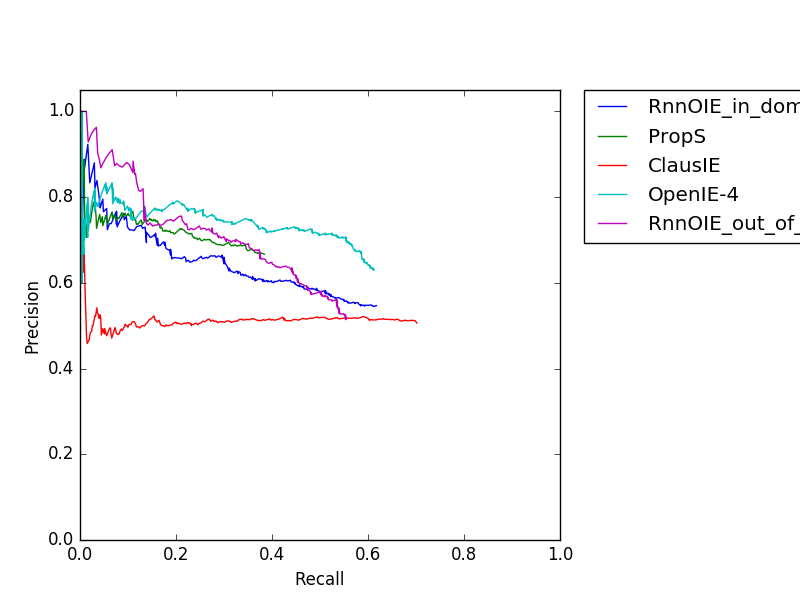
\includegraphics[width=\textwidth]{figures/newswire/pr}
%%       \caption {Precision-recall curve on the newswire test partition}
%%       \label{fig:alignments}
%%     \end{center}
%%   \end{minipage}


%% \end{figure*}
